\section{Gibbs and the Reification of Vectors: From Geometry Back to Calculation}

If Riemann revealed that space itself could curve,  
and Cayley abstracted geometry into algebra,  
and Fourier decomposed phenomena into modes,  
then Josiah Willard Gibbs gave scientists a way to calculate with these abstractions in their hands.

Where Riemann turned geometry into a field of tensors and manifolds,  
Gibbs brought geometry back to the working desk of the physicist—  
transforming mathematical abstraction into a usable calculus for fields, forces, and flows.

\bigskip

\subsection*{The Leap from Riemann to Gibbs}

Riemann had given us a vision: space as a manifold, geometry as curvature, distances defined intrinsically by a metric.

But in the 19th century, physics still operated largely in the Euclidean world of three-dimensional space.

Physicists needed tools to work with fields, forces, and rotations—  
to describe electromagnetism, fluid dynamics, and mechanics without drowning in the expanding notational machinery of quaternions or matrix algebras.

It was here that Gibbs intervened.

He recognized that while quaternions (popularized by Hamilton) offered a four-dimensional algebraic system,  
physicists mostly needed operations in **three dimensions**—dot products, cross products, gradients, divergences, curls.

Gibbs stripped the machinery down to what was essential.

He introduced **vector analysis**: a system where vectors could be manipulated by clear operations tied directly to physical meaning:

\[
\vec{A} \cdot \vec{B}, \quad \vec{A} \times \vec{B}, \quad \nabla \cdot \vec{F}, \quad \nabla \times \vec{F}
\]

\bigskip

\begin{tcolorbox}[colback=gray!5!white, colframe=black, title=\textbf{Sidebar: The Shift from Riemann to Gibbs}, fonttitle=\bfseries, arc=1.5mm, boxrule=0.4pt]

\begin{tabular}{>{\raggedright}p{4cm} >{\raggedright}p{5.5cm} >{\raggedright\arraybackslash}p{5.5cm}}
 & \textbf{Riemann} & \textbf{Gibbs} \\
\midrule
Key object & Metric tensor defining geometry at each point & Vector operators defining fields in \( \mathbb{R}^3 \) \\
Geometry as & Intrinsic property of manifold & Practical tool for physics in Euclidean space \\
Focus & Curvature, geodesics, tensor fields & Gradients, divergences, curls; operations on vectors
\end{tabular}

\end{tcolorbox}

\bigskip

\subsection*{From Curvature to Calculation}

Where Riemann envisioned spaces bending under curvature,  
Gibbs gave a language to describe the flow of water through a pipe,  
the rotation of a magnetic field,  
the divergence of an electric field from a point charge.

In Gibbs’s vector analysis, physicists could manipulate fields algebraically without invoking coordinates explicitly.  
They could calculate work, circulation, flux, and potential with a symbolic toolkit directly mirroring physical intuition.

In a sense, Gibbs’s leap was a move from **geometry back to calculation**—  
from the grand structures of curved manifolds to the **pragmatic structures of fields living inside \( \mathbb{R}^3 \).**

\bigskip

\subsection*{A Bridge Between Abstract and Applied}

Gibbs didn’t negate Riemann’s geometry; he gave physicists a working interface with it,  
before tensor calculus became widespread.

His vector analysis acted as a bridge between the geometric abstraction of curvature  
and the hands-on algebra needed for Maxwell’s equations, thermodynamics, and mechanics.

Where Fourier decomposed functions, Gibbs decomposed physical phenomena into components aligned with human measurement—along, across, rotating around.

And where Cayley encoded transformations algebraically, Gibbs encoded physical operations algebraically.

\bigskip

\begin{quote}
In Euler, we computed forces.  
In Lagrange, we minimized action.  
In Hamilton, we traced flows.  
In Jacobi, we found surfaces.  
In Cayley, we abstracted transformations.  
In Fourier, we decomposed vibrations.  
In Riemann, we curved the space.  
In Gibbs, we brought geometry back into the laboratory.
\end{quote}

\subsection*{Setting the Stage for Tensors and Fields}

Gibbs’s system made the manipulation of vectors intuitive,  
but the world would soon require more:  
tools capable of describing fields not just in \( \mathbb{R}^3 \), but in curved spacetime itself.

The simplicity of Gibbs’s dot and cross products would generalize into the tensor calculus of Ricci and Levi-Civita,  
where operations had to work across coordinates that bent and twisted under curvature.

But before tensors were universal, Gibbs gave physicists the algebra they needed to tame vectors.

And in doing so, he laid a practical foundation that would echo even in the curved geometries of Einstein’s universe.


\subsection*{Reinterpreting Kepler’s Second Law Through Gibbs’s Vector Analysis}

Gibbs brought physics back to the chalkboard — and with it, a notation that made celestial mechanics calculable in three dimensions.

Kepler’s Second Law — that a planet sweeps out equal areas in equal times — can now be understood not just as a geometric principle or a curvature-induced symmetry,  
but as a direct consequence of a conserved quantity in vector form.

\bigskip

\begin{tcolorbox}[colback=blue!5!white, colframe=blue!70!black, title=\textbf{Gibbs’s View: Kepler as a Vector Conservation Law}]
In Gibbs’s language, Kepler’s Law is the constancy of the areal velocity vector:
\[
\vec{L} = \vec{r} \times \vec{v}
\quad \text{with} \quad
\frac{d\vec{L}}{dt} = 0
\]
\end{tcolorbox}

\bigskip

\paragraph{From Area Sweep to Angular Momentum.}

The areal velocity swept out by the planet is given by:
\[
\frac{dA}{dt} = \frac{1}{2} \left\| \vec{r} \times \vec{v} \right\|
\]

This is precisely half the magnitude of the angular momentum per unit mass:
\[
\vec{L} = \vec{r} \times m\vec{v}
\]

In Gibbs’s formalism, this isn’t just a geometric fact — it’s an algebraic identity.  
The cross product encodes both the direction of orbital motion and the plane in which the motion is confined.

\bigskip

\paragraph{Why the Cross Product Matters.}

Thanks to Gibbs, we now treat the cross product as a fundamental tool in physics.  
And Kepler’s Law becomes a perfect example of its meaning:

\begin{itemize}
    \item The direction of \( \vec{r} \times \vec{v} \) is perpendicular to the orbital plane,
    \item The magnitude measures twice the areal velocity,
    \item Its conservation implies that no torque acts perpendicular to the plane.
\end{itemize}

In short, the vector remains constant — and that constancy is the Second Law, expressed with precision and power.

\bigskip

\paragraph{From Geometry to Calculation.}

What had once required diagrams and proportional reasoning,  
Gibbs now lets us express in a single algebraic condition:

\[
\vec{r} \times \vec{v} = \text{constant}
\]

This equation is compact, visualizable, and computationally tractable — a gift to physicists navigating real-world orbits.

\bigskip

\begin{quote}
Kepler drew ellipses.  
Newton explained forces.  
Gibbs wrote: \quad \( \vec{r} \times \vec{v} = \text{const} \)  
And every physicist since has smiled.
\end{quote}

\begin{figure}[H]
    \centering
    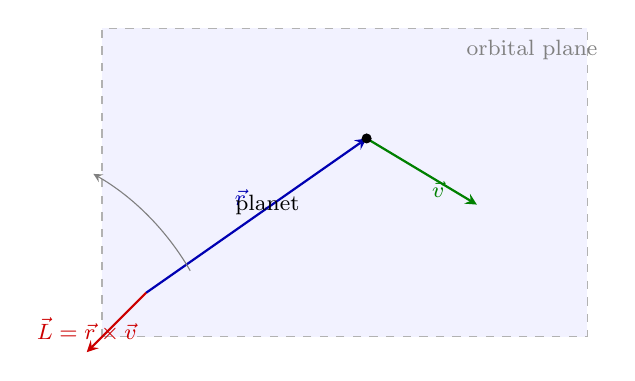
\begin{tikzpicture}[scale=2.8, >=stealth]
    
      % Origin and axes
      \coordinate (O) at (0,0);
      \coordinate (R) at (1,0.7);  % r vector
      \coordinate (V) at (1.2,0.2); % v vector
      \coordinate (L) at (0,0,1); % angular momentum vector (out of plane)
    
      % Draw orbital plane
      \fill[blue!5] (-0.2,-0.2) rectangle (2,1.2);
      \draw[black!30, dashed] (-0.2,-0.2) rectangle (2,1.2);
      \node[black!50] at (1.75,1.1) {\footnotesize orbital plane};
    
      % Vectors
      \draw[->, thick, blue!70!black] (O) -- (R) node[midway, above left] {\footnotesize $\vec{r}$};
      \draw[->, thick, green!50!black] (R) -- ++(0.5,-0.3) node[midway, below right] {\footnotesize $\vec{v}$};
      \draw[->, thick, red!80!black] (O) -- (0,0,0.7) node[above] {\footnotesize $\vec{L} = \vec{r} \times \vec{v}$};
    
      % Add circular arc to show motion
      \draw[black!50, ->] (0.2,0.1) arc[start angle=30, end angle=60, radius=1.2];
    
      % Labels
      \node at (0.55,0.4) {\footnotesize planet};
      \filldraw[black] (R) circle (0.02);
    
    \end{tikzpicture}
    \caption{Visualization of Kepler’s Second Law using Gibbs’s vector notation. The cross product $\vec{r} \times \vec{v}$ yields a constant angular momentum vector perpendicular to the orbital plane.}
    \end{figure}
    